%%%%%%%%%%%%%%%%%%%%%%%%%%%%%%%%%%%%%%%%%%%%%%%%%%%
%% P3: Phenomenology of Particle Physics                         
%%
%% Author:  André Rubbia                   		 
%%
%% Figure 26.6 The asymmetry parameter as a function of the Weinberg mixing angle.
%%
%% This work is licensed under the Creative Commons Attribution 4.0 International License. 
%% To view a copy of this license, visit http://creativecommons.org/licenses/by/4.0/ or 
%% send a letter to Creative Commons, PO Box 1866, Mountain View, CA 94042, USA.
%%
%%%%%%%%%%%%%%%%%%%%%%%%%%%%%%%%%%%%%%%%%%%%%%%%%%%

\documentclass[a4paper,10pt]{article}

\usepackage[T1]{fontenc}
\usepackage[utf8]{inputenc}
\usepackage{lmodern}
\usepackage[labelfont=bf]{caption}
\usepackage{upgreek}

\usepackage{tikz}
\usepackage{pgfplots}
\pgfplotsset{compat=1.17}
\usepgfplotslibrary{ternary}
\usepgfplotslibrary{fillbetween}
\usepgfplotslibrary{external}

\def\d{\mathrm{d}}
\setlength{\oddsidemargin}{-1.0cm}
\setlength{\evensidemargin}{-1.0cm}
\setlength{\textheight}{25cm}
\setlength{\textwidth}{18cm}

\begin{document}

%%%%%%%%%%%%%%%%   FIGURE  %%%%%%%%%%%%%%%%%%%%%%%%%%%%%%
\begin{figure}[htb]
\centering
\begin{tikzpicture}[scale=1.]
\begin{axis}[xmin=0, xmax=1,
	xtick={0,0.5,1},
	ymin=-1, ymax=1,
	title=$Z^0$ asymmetry parameter,
	xlabel=$x_W \equiv \sin^2\theta_W$,
	ylabel=${\cal A}_f$,
	xmajorgrids=true,
	ymajorgrids=true,
	legend entries={${\cal A}_\ell$,${\cal A}_{u,c,t}$, ${\cal A}_{d,s,b}$},
	legend pos = north east
]
	\addplot[domain=0:1,blue,very thick, samples=100] {2*(1-4*x)/(1+(1-4*x)^2)};
	\addplot[domain=0:1,blue,very thick, samples=100,dashed] {2*(1-8/3*x)/(1+(1-8/3*x)^2)};
	\addplot[domain=0:1,blue,very thick, samples=100,dotted] {2*(1-4/3*x)/(1+(1-4/3*x)^2)};
	 \draw[red, very thick, dashed] (axis cs:0.23,-1) -- (axis cs:0.23,1);
\end{axis}
\end{tikzpicture}
	\caption{The asymmetry parameter as a function of the Weinberg mixing angle. The vertical
	dashed line indicates the value $x_W=0.23$.}
	\end{figure}
%
%%%%%%%%%%%%%%%%   END FIGURE  %%%%%%%%%%%%%%%%%%%%%%%%%%%%%%
%
\end{document}
